\documentclass[12pt,twocolumn,twoside]{conference}   %%
\usepackage[german, english]{babel}                  %%
%%% Vorgaben %%%%%%%%%%%%%%%%%%%%%%%%%%%%%%%%%%%%%%%%%%


\title{Technique and procedures of business analytics}

\author{}

\begin{document}
\twocolumn[
  \begin{@twocolumnfalse}
  \maketitle\thispagestyle{firststyle}
    \begin{abstract}
    \vspace{8pt}
Business Analytics is a kind of tool for the area of controlling in a company. The tool will be used to solve future problems based on past information.
This paper deals with these business analytics and their comprehensive procedures, approaches and methods. First, we report on what business analytics are. This is followed by an analysis of a possible, structured approach to business analytics and how it can be structured. Subsequently, the procedure of the so-called Knowledge Discovery in Databases (KDD) will be discussed and there especially the Data Mining. Finally, predictive analytics and the methodological and architectural approaches to be recommended are presented.
    \end{abstract}
    \vspace{16pt}
  \end{@twocolumnfalse}
]

\section{Business Analytics}
\subsection{Business Analytics - Introduction}
In the past, it was the task of a so-called controller to juggle the figures and thus to check and reproduce the economic figures of a company. But nowadays this has changed. The field of activity of a controller has become much more complex and technically adept in the last decades. Nowadays, one of the main tasks of a controller is to apply so-called "business analytics" in order to keep the company economically, so that it can still be represented on the market. But what exactly are these business analytics?
In order to provide a better insight into business analytics, the following questions are answered first: 

\begin{enumerate}
\item What exactly are business analytics?
\item What is the general procedure for business analytics?
\item Why do you use business analytics?
\item Why is so much attention paid to business analytics?
\item fields of application of business analytics
\item What has to be considered with business analytics?
\item What kind of analysis tools are available for business analytics?
\end{enumerate}

\subsection{What are business analytics?}
Business analytics is the process of researching and evaluating historical data for the future orientation of the company.  As already described above, they are mainly seen as a kind of tool of the controller. With the help of business analytics, historical data of the company or the data of the company environment are used to make decisions as to what course the company should take in order to be able to operate economically in the future as well. It is important to understand that business analytics is an ongoing process that is divided into several phases. This is described with in the following subarea.


\subsection{Business Analytics - General procedure}

\begin{figure}[H]
\centering
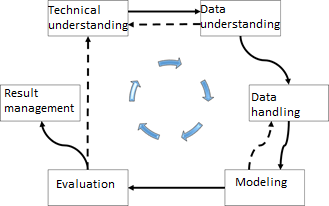
\includegraphics[width=8cm]{Abbildungen/Business_Analytics_Process.png}
\caption{Business Analytics Process}\label{visina8}
\end{figure}

This ongoing process described above can be interpreted in such a way that the controller needs a certain technical understanding in order to develop a feeling for the relevant data. These can and should be adjusted after changes in market conditions, changes in internal or external structures, or even from time to time. Depending on the situation, the data to be fed into the analysis are now prepared and modeled. Here, too, it is possible that the data used to model the analysis may have to be adjusted several times. Once the modeling is complete, the results of the analysis are evaluated. Now it may be that these results are not helpful or do not provide enough information for the current situation. If this is the case, the technical understanding is prepared and deepened again. It is also possible that the technical understanding benefits from the results of the evaluation and that a further, more detailed analysis can be started on the basis of this. However, if the original analysis delivers desired or meaningful results, these are now distributed or passed on so that the company can take the next steps to optimize profitability. Finally, the described analysis process is applied to another area of the company in need in order to optimize the effectiveness of this area.

\subsection{Why do you use Business Analytics?}
Unfortunately, the question why business analytics is used cannot be answered in one sentence. Business analytics is used to analyze, evaluate and finally evaluate large amounts of data, or "big data". A great advantage of this method is that even non-uniform, heterogeneous data can be optimally structured and evaluated. Thanks to this evaluation, it is possible, for example, to interpret and analyse the consumer behaviour of buyers and, in the best case scenario, find out that if you can reduce the production costs of the best-selling product through intensive research, and thus generate more profit. The mentioned example is only one possible application. Of course there are many more here. In summary, it can be said that the use of business analytics, and the market research generated by it, for example, can and will have a positive effect on the companies that uses them correctly.

\subsection{Wieso werden Business Analytics so viel Aufmerksamkeit gewidmet?}
The concept of Business Analytics, which is based on the principle of Business Intelligence, is definitely not a new publication. The first approaches of Business Intelligence were already published in the late 1950s (vgl. Punkt 3 aus txt) and dealt with the continuous data collection within a company. So why is this issue still receiving so much attention today? On the one hand, because the basic idea has changed from Business Intelligence to Business Analytics. This means that data is no longer simply to be recorded and managed; instead, it is also evaluated appropriately and professionally and, in the best case, future events are predicted.  On the other hand, because today's technological state offers many more possibilities. Since then, the computing power alone has increased by at least a factor of 1000, not to mention the capacities of the storage media.  For example, it is theoretically possible to implement the business analytics approach described above completely by combining hardware and software, which delivers useful results in the shortest possible time.

\subsection{Business Analytics - Application Areas}
If a company has decided to perceive business analytics as a point of optimization, it must check for the right methods and algorithms. Furthermore, it must be examined what kind of business analytics system will be useful in the company. To this end, Mehenna et al divide the fields of application of business analytics into the following five areas:

\begin{itemize}
\item Analysis
\item Forecast
\item Optimization
\item Simulation
\item Radar
\end{itemize}

These 5 fields of application allow the Business Analytics System to exploit the full potential if these fields of application interact (cf. Mehenna et al. 2016) 

\subsubsection{Application Area - Analysis}
The basis of all business analytics systems is to run an analysis on existing historical data. Here the field of application of the analysis is seen as a process, which implies that knowledge is gained from the individual structural properties of the data. What kind of big data analysis method is used varies from target to target. The analysis procedures will be further explained later in the paper. The aim of the field of application of the analysis is to answer questions. 

\begin{@twocolumnfalse}
\begin{figure}[H]
\centering
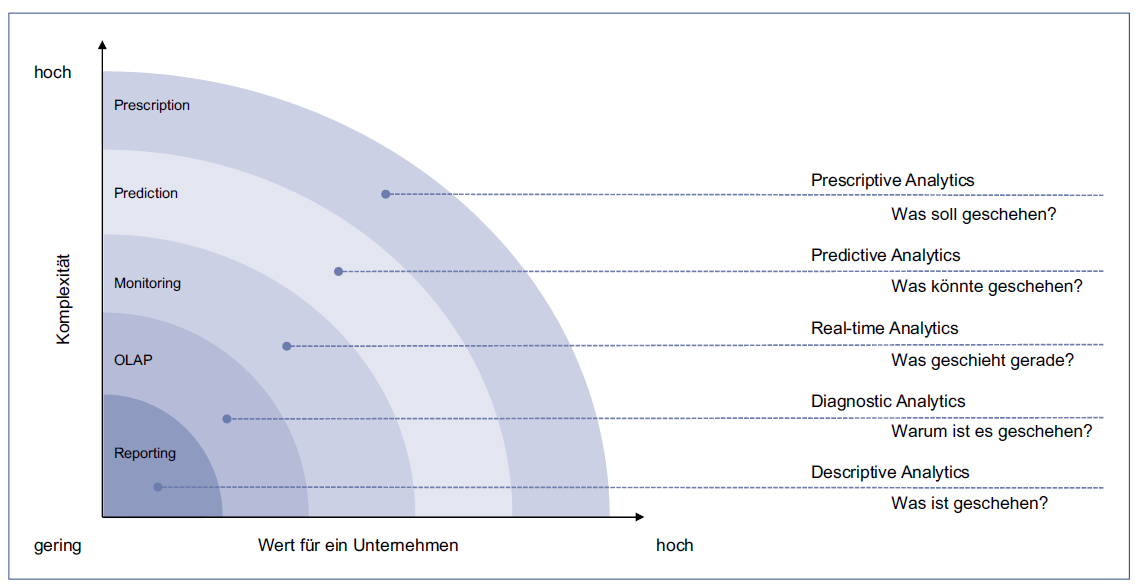
\includegraphics[width=20cm]{Abbildungen/Analysis.png}
\caption{Analysis Questions}\label{visina8}
\end{figure}
\end{@twocolumnfalse}

As Figure 2 can be taken from, the questions that can be asked and answered are each a different solution of the Business Analytic System. Within the scope of the field of application of analysis, however, only descriptive analytics, diagnostic analytics and real-time analytics are used. The descriptive analytics follow the classical reporting, where it is analyzed afterwards, what has happened and when. did it happen. Diagnostic Analytics follows the investigative approach. The main question here is why this situation could have arisen. The last shown possibility of the application field of analysis corresponds to the principle of real-time analytics. These are based on monitoring systems which are currently in operation. 

\subsubsection{Application Area - Forecast}
Forecasting is a business analytics tool that uses stochastic models, machine learning and data mining approaches to make efficient forecasts with good results (vgl Mehanna, 2016). Here, too, there is an additional distinction to the so-called digital forecasts. The digital forecasts can be used in such a way that at the end, for example, by combining several of these digital forecasts, to forecast the so-called EBITDA (earnings before interest, taxes, depreciation and amortization). In this example, the following forecasts have been combined. First, the "sales forecasts based on unstructured data on trends". In addition, a forecast for "fully automated pricing". This is followed by an "early detection of changes in raw material prices" and last but not least, one for "optimization of warehousing" (cf. Mehanna et al. 2016). The result is a continuously learning sales forecast. 

\subsubsection{Application Area - Optimization}
With the help of forecasts or digital forecasts you now get information about the future development of the areas on which the forecasting was applied. Of course, this alone is not enough to allow the company to operate more economically. Another important factor is optimization. The optimization procedure follows the forecasting procedure. A very good example of optimization is that of optimizing the inventory in the retail trade. Here the system is automatically adjusted so that, when a customer orders an article, it is automatically offset against the stock quantity of the article in the warehouse. As soon as a predefined minimum is reached, this article is at best automatically reordered by the system (see Mehanna et al. 2016). The model explained in this example reduces both the cost of the company's stock and the cost of ordering new goods. However, not the actual cost of the goods. Models for identifying new cause-effect relationships can be continuously developed and thus generate new insights into bottlenecks or inefficiencies. On the other hand, automated analyses shorten reaction times, enable "high-frequency decisions" and lead continuously to ad-hoc implementation of optimization measures.'\cite{PAPER2}. The focus of the optimization process is on the continuous optimization of the overall system.

\subsubsection{Application Area - Simulation}
The simulation process describes the simulation of a company and possible future developments. Various scenarios for possible corporate development are already being simulated today, for example in the context of corporate planning. At present, however, most of these simulations are characterized by high manual effort and personnel commitment. In addition, the short-term response to changes in the scenarios is very limited. As a result, simulations for corporate management are often reduced to a minimum and thus cannot unfold their added value. potentially highly relevant control information will be lost.'. \cite{Mehanna et al. 2016}. What Mehanna is talking about is that the simulations often do not offer enough meaning, attention and resources of any kind. If they were properly designed and fed with all data relevant to the simulation, they could be used to support operational decisions. For this type of simulation, there are driver-based models, such as the revenue control model. The aim of the revenue management model is to ensure that the available resources of all kinds generate the highest revenue. In the best case, the business analytics forecast is the basis of this model. All relevant data, such as capacity, prices, load, operating time, etc., are loaded into the revenue control model. The results of this simulation are, for example, optimized prices at certain selling points (see Mehanna et al. 2016). It should be noted here that the simulation is a kind of learning algorithm and that in the best case this should also be fed with actual values so that these are taken into account in the forthcoming simulations. 


\subsubsection{Application Area - Radar}
The radar method is the continuous observation and analysis of the market segment in which the company operates. This is where the term competitive intelligence comes into play. Competitive intelligence combines processes and technologies for clarifying the market and its associated components, such as patents, customers, suppliers, competitors, etc. (cf. Mehanna et al. 2016). The basis for useful data that can be fed into the radar are social media channels and, in general, everything that can be understood by "open data". Open Data includes public sites as well as forums and websites of different companies in the same market segment. This information is analyzed using semantic analyses. These include methods such as Natural Language Processing or Text Mining. Furthermore, all relevant information or findings should be obtained in the radar procedure. These can help a company to make its own brand more competitive, since it can also evaluate external characteristics, such as the perception of its own brand by a customer. Thanks to radar, more resources can nowadays be invested in innovations, which explains the current growth in product diversity.

\subsubsection{Application Area - Résumé}
As already mentioned, Business Analytics is an extended methodological and technological toolbox for the area of controlling. The 5 fields of application are for orientation and should definitely not be considered individually. In an enterprise, ideally, these fields of application should be linked and it would even make sense to integrate a system that contains a combination of all five fields of application. However, at the beginning, care should be taken to examine the application field systems individually and gather experience with them before integrating another application field system. 

\subsection{What has to be considered with Business Analytics?}
So far, this paper has only reported positively from Business Analytics. Then how come not every company works with business analytics? One of the reasons is that the investment in the technology itself is relatively expensive and does not solve all problems. It is also important that the users must be able to limit the problems and then run their analyses on them. Only those who provide the right data for analysis in advance will possibly arrive at useful results. Furthermore, it is not only relevant which data is made available for analysis, but also with which algorithm it is processed. Additionally, the style of visualization of the results is added. As long as these are not presented in a meaningful way, the most effective algorithms and the best data are useless. Last but not least, it is always the final interpretation of the competent authority. As can be concluded from this, there are also a considerable amount of risks in business analytics. So how should business analytics be used? Carsten Felden explained it in his blog as follows: 'First of all, when introducing business analytics, the added value for the company must be determined, since the benefits acquired must justify the effort. Another facet is the underlying project-oriented and process-oriented approach. The project-oriented characteristic results from the fact that it is in the nature of data mining approaches, for example, not to be a control loop. New data must be compiled for the respective value-creating tasks, goal-oriented analysis options for the underlying data must be evaluated and executed in order to be able to use the results in daily business operations.'. \cite{Beispiel1:2016} As the text by Carsten Felden shows, it should first be considered whether the area of application of the company reflects any benefit for business analytics or not. It is then important that the system is or can be permanently supplied with meaningful information. If these points do not speak in favour, the company should not opt for a solution approach based on business analytics.

\subsection{What analysis tools are available for Business Analytic?}
Since business analytics is more an approach than a concrete solution, there are various analysis tools. Here are some of the most popular:

\begin{itemize}
\item A/B tests
\item Statistical or quantitative analysis
\item Text Mining
\item Data Mining
\item Predictive Analytics
\end{itemize}

While A/B tests, statistical or quantitative analysis and data mining are already quite precise approaches to plan a company's future course, predictive analytics is again a subfield of business analytics. The following chapters will describe data mining and predictive analytics.

\section{Knowledge Discovery in Databases(KDD) }
\subsection{KDD - Introduction}
In the course of business analytics, there are many methods and tools to analyze and later evaluate large amounts of data. It is not a big problem to evaluate data which only change in the individual values. But what if the data has an uneven structure? For the just mentioned case, the so-called heterogeneous data, there is the method of knowledge discovery in Databases, Which is often confused with data mining. 

\subsection{KDD - Process}
Basically, data mining is a partial step, namely that of data analysis and knowledge discovery in databases processes. The aim of the KDD is the recognition of so far unknown technical connections from existing, mostly large data sets. In contrast to data mining, KDD also includes the preparation of the data and the evaluation of the results as an overall process.'. \cite{Beispiel:2016}

\begin{figure}[H]
\centering
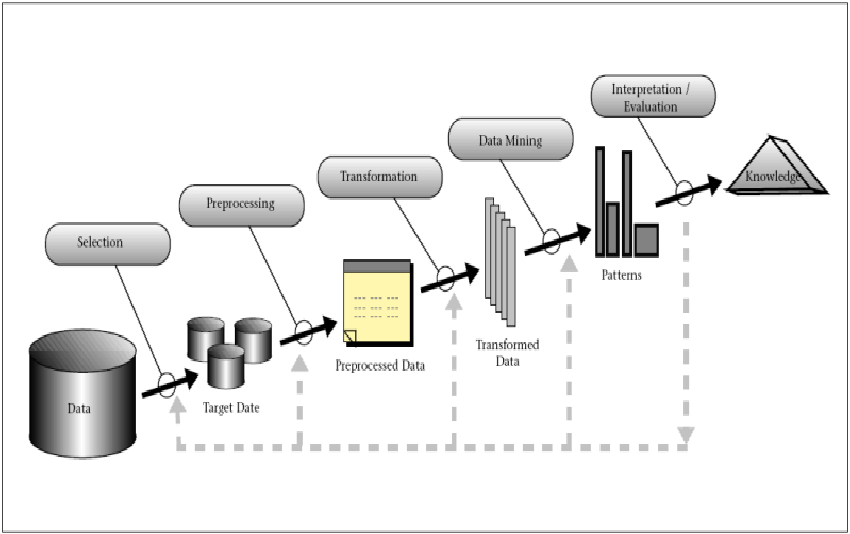
\includegraphics[width=8cm]{Abbildungen/KDD.png}
\caption{KDD Process}\label{visina8}
\end{figure}

As Figure 3 shows, the KDD process consists of several steps. The first step, the selection step, which consists of first picking out those data that could have a meaning for the analysis to be carried out. These are then preprocessed, where erroneous data is removed or corrected. What follows is the process of data reduction, in which the data is reduced to the data content which is going to be processed. Then follows the step of data mining, in which the actual data analysis is performed. The result of this analysis is pushed into different, previously selected patterns which are finally be ready to be evaluated and interpreted by the user.


\subsection{KDD - Data Mining Application Procedures}
The procedures in which a data mining application works differ from company to company and even here from situation to situation depending on the wanted outcome. The typical procedures are essentially divided into the following (8. Im Dokument):

\begin{itemize}
\item Anomaly analysis
\item Cluster analyses
\item Classification
\item Association analyses
\item Regression analysis
\end{itemize}

\subsubsection{Anomaly analysis}
Anomaly analysis is a type of analysis in which an average is formed and any data set that differs too much from this average is marked as suspicious. It is usual that data records marked as suspicios are manually checked for correctness by a user.

\subsubsection{Cluster analyses}
In so-called cluster analyses, the data sets are analyzed in certain concentrations within a data room. If a data set does not fit into a cluster, it is marked as suspicious, depending on the type of procedure, as in anomaly analysis. Here too, data records marked as suspicious are checked for correctness by a user.

\subsubsection{Classification}
Similar to cluster analyses, the data records are analyzed and mapped into a data room when classifying data. However, unlike cluster analysis, these rooms are predefined before the analysis procedure. 

\subsubsection{Association analyses}
Die Assoziationsanalysen suchen Normalität bzw. Regelfälle in den Datensätzen. Diese Ergebnisse könnten zum Beispiel angeben, welche Art von Objekten in irgendeiner Art und Weise in Relation zueinander stehen. 

\subsubsection{Regression analysis}
The association analyses search for normality or rule cases in the data sets. These results could, for example, indicate what kind of objects are related to each other in some way. 

\subsection{KDD - Data Mining specializations}
A frequently used algorithm for big data analysis is data mining. However, since there are an unmanageable number of further possibilities to analyze other data types, the data mining algorithm has also produced special modifications. These specializations start where the normal data mining algorithm reaches its limits. Since there is a different data mining algorithm for almost every different data type, only a few are mentioned here. On the one hand, there is text mining, which is an analysis procedure that analyzes textual data. With data mining, text mining is probably one of the best-known analysis methods. An example application is represented in the so-called plagiarism determination. Another specialized modification is the so-called web mining. Web mining is based on the algorithms of cluster analysis and association analysis. This is used by some search engines, for example. 

\subsection{KDD - Conclusion}
Finally, it can be said that the purpose of data mining applications is to uncover non-trivial patterns in larger amounts of data. The resulting models are usually applied to current or future data constellations in order to extract information from the analysis.

\section{Predictive Analytics}
\subsection{Predictive Analytics - Introduction}
Predictive analytics is a process that uses and evaluates historical data to predict future events. In contrast to knowledge discovery in databases, predictive analytics is not only about evaluating the data and using this evaluation to initiate the next steps, but rather about generating models for evaluation using the data (vgl. Baars et al. 2016). 

\subsection{Predictive Analytics - Methodical aspects}
Since predictive analytics focuses on predicting future events, there are also a few methodological requirements for the process. On the one hand, it depends on where the information used for analysis comes from. In doing so, care should be taken to ensure that only trustworthy information from the immediate environment or data/information collected oneself is used. It is also important that the end user who evaluates the results is also shown the final values of the analysis in addition to the results. On the other hand, it is important that the methods used to carry out the analysis take into account the market environment or the industry. One of the methodological peculiarities is that the system is both modeled from the user's point of view and predefined connections and restrictions so that the system can work effectively for the respective application (vgl. Dr. Baars 2016).

\subsection{Predictive Analytics - Architectural Aspects}
With a predictive analytics system, it is recommended to use several systems that are responsible for the analysis. For these purposes, it would make sense to operate a system separate from the production system in the form of a sandbox. Furthermore, it requires high-quality data to generate models. This data, relevant for analysis and model generation, should be both internal and external in nature. For the sandbox system it is also recommended to have a number of tools available, for example data mining tools as well as data manipulation and data integration tools (see Dr. Baars 2016). The combination of all these technical aspects serves to be able to observe an analysis process and to transfer the resulting information and experience into the production system. 

\section{Conclusion}
Business analytics and especially knowledge discovery in databases and predictive analytics are approaches that could appeal to every IT industry, since the digitization of corporate management with big data and business analytics could trigger a paradigm shift (see PAPER 2). There it makes no difference whether it is used in a normal retail trade or in banks. Each of these sectors could benefit tremendously from a correctly implemented business analytics system. Then why hasn't it been implemented everywhere? Costs are a big argument against business analytics. The costs involved in setting up a complete business analytics system with all components are immensely high. Furthermore, a certain amount of time must first pass under observation before the system can belong to the production system. The last and most important point, however, is still that of the controlling personnel. In the end, it does not matter how the system was implemented, if the staff evaluates or interprets the results of the analysis "incorrectly", it may be that a company takes a wrong course and the profitability of the company will suffer as a result. Another problem is that data-driven control is far from being perfected. However, there are also a lot of positive examples of the use of business analytics and more precisely the use of predictive analytics. For example, the global player IBM has been using predictive analytics for years and even offers services and tools for company optimization purposes. In my opinion, although the whole issue should be treated with caution, it is definitely worth continuing to be monitored.  
\newpage

\begin{thebibliography}{99}
	\bibitem{Beispiel1:2016}
	Beispiel1: http://www.enzyklopaedie-der-wirtschaftsinformatik.de/lexikon/daten-wissen/Business-Intelligence/Analytische-Informationssysteme--Methoden-der-/Business-Analytics 
	Aufgerufen am 23.06.2018 um 15:37 Uhr CEST
	\bibitem{PAPER2}
	Beispiel2: https://de.wikipedia.org/wiki/Knowledge-Discovery-in-Databases
	Aufgerufen am 19.06.2018 um 11:54 Uhr CEST
	\bibitem{ISO9075-1:2011}
	ISO/IEC 9075-1: Information technology
	Database languages -SQL- ,Part 1: Framework
	(SQL/Framework), 4. Auflage, ISO Copyright Office,
	Genf 2011
\end{thebibliography}

\end{document}
